\documentclass[12pt]{article}
\usepackage[english]{babel}
\usepackage{graphicx}
\usepackage{hyperref}
\usepackage[utf8]{inputenc}
\usepackage{fancyhdr}

\pagestyle{fancy}
\fancyhf{}
\lhead{Uppsala University}
\cfoot{\thepage}
\rfoot{Thameez Bodhanya}
\renewcommand{\headrulewidth}{0.5pt}
\renewcommand{\footrulewidth}{0.5pt}

\begin{document}

\begin{titlepage}

\begin{figure}
   \begin{minipage}{0.48\textwidth}
   \begin{flushleft}
     
\includegraphics[scale=0.5]{Images/UU_LOGO.png}
   \end{flushleft}
   \end{minipage}\hfill
   \begin{minipage}{0.48\textwidth}
   \begin{flushright}
     
\includegraphics[scale=0.075]{Images/Allan Gray.png}
   \end{flushright}
   \end{minipage}
\end{figure}

\thispagestyle{fancy}

\vspace{1in}

\center

\textsc{\large MASTER THESIS SPECIFICATION}

\vspace{0.5in}

\noindent\makebox[\linewidth]{\rule{\linewidth}{1.2pt}}
\textsc{ \textbf{\large Investigating Impact, Performance, and Suitability of Cloud Orchestrated Container Platforms}}
\noindent\makebox[\linewidth]{\rule{\linewidth}{1.2pt}}

\vspace{0.5in}

\begin{minipage}{0.48\textwidth}
    \begin{flushleft}
        \textit{Student:} \\
        Thameez Bodhanya \\
        thameez.bodhanya.4249@student.uu.se
    \end{flushleft}
\end{minipage}
\begin{minipage}{0.48\textwidth}
    \begin{flushright}
    \textit{Supervisor:} \\
    Calvin Moore \\
    calvin.moore@allangray.co.za
    \end{flushright}
\end{minipage}

\vspace{2in}

\textbf{\large Department of Information Technologies} \\

\today

\end{titlepage}

\newpage

\setcounter{page}{2}
\tableofcontents
\newpage

\section{Title}
 Investigating Impact, Performance, and Suitability of Cloud Orchestrated Container Platforms

\section{Background}

Containerization (or OS-Level Virtualization) \cite{virtualization} revolutionized the business world in 2013 with the introduction of Docker \cite{docker}. Coupled with the high adoption rate of containerization saw the rapid adoption of container-orchestration tools (with the most popular being Kubernetes\cite{k8s}).

In parallel to the adoption of the aforementioned technologies, cloud-computing providers matured from offering basic compute, storage, and networking offerings; to more managed "cloud-native" services. 
Amazon Web Services (AWS), for example announced an early version of their custom container-orchestration tool (ECS) in 2015 \cite{ecs}, expanding their container-orchestration offerings with a serverless container platform (Fargate) in 2017\cite{fargate}, and a managed Kubernetes Engine (EKS) in 2018 \cite{eks},. More recently, AWS has announced the ability to run containers as Lambdas (Serverless Functions) in late 2020\cite{lambda}.

\noindent These shifts in technological maturity enables workloads to fully leverage the advantages of containerization, with those offered by the cloud. 
Unfortunately, the partition between the cloud offered container platforms are not entirely clear and rather fuzzy (this includes performance, security, efficiency, latency and cost).\\

\noindent Allan Gray is no exception to the above scenario. Allan Gray has been running container workloads in production for over five years, running on the Kubernetes platform, on an on-premise data-center on virtual Linux machines. 
Allan Gray is currently undertaking a cloud-migration, and is looking to shift their container-workloads to the cloud (with AWS being their chosen cloud platform). 
As such, Allan Gray requires an environment in the cloud which runs various types of services as containers which can communicate with each other, the outside world, on-premise services, and other AWS services; in a secure manner. The environment should be easily tracked and measured using metrics at every level. Their current deployment mechanism should not require major tooling changes, or a steep learning curb. The proposed solution should meet security and risk measures.\\

\noindent This project aims to investigate the various options available, in terms of:
\begin{itemize}
    \item ease of adoption and configuration
    \item deployment process
    \item restrictions and limitations 
    \item performance 
    \item cost impacts
    \item reliability and resilience  
    \item security and audit 
\end{itemize}

\noindent To achieve this goal, an investigation of current tools, designs, and architectures used at Allan Gray would be required. The result of this investigation would be both a general analysis of the proposed solutions, and a specific solution catered to the constraints of \textit{Allan Gray}.

\subsection{Why AWS?}
Whilst it seems that experimenting only on AWS severely restricts the generality of this investigation, in reality the offerings by the other two major cloud providers (being Google Cloud Platform and Microsoft Azure Cloud respectively), match the Cloud Orchestrated Container offerings by AWS at a feature-parity level \cite{contaier_workloads}. 
Additionally, AWS holds more that 33\% of the cloud market (as of Q4 2021) \cite{aws_cloud_share}, and is considered to be the cloud-provider of choice for the the largest tech companies in the world today \cite{aws_users}. 

Therefore the results of this investigation (and recommendations) would (in theory) apply to the GCP and Azure cloud as well.

\section{Description of Tasks}
This project will be split into three major tasks:
\subsection{Research}
This task will focus on
\begin{itemize}
    \item investigating best practices/current recommendations according to research 
    \item understanding \textit{Allan Gray}'s requirements and current processes
    \item understanding the current metrics being exposed (and tooling)
    \item identifying designs/architectures which meet the requirements of this project 
    \item fully documenting and understanding the various solutions available 
    \item ensure that security best-practices are being followed (both in terms of system security and privacy)
\end{itemize}
\subsection{Experimentation}
This task will focus on defining and measuring the differences between each viable option under the metrics of:
\begin{itemize}
    \item cost
    \item performance and latency 
    \item resilience and reliability 
    \item ease-of-use
\end{itemize}.
\subsection{Design and Implementation}
This task will focus on using the results of the above research and experimentation to implement and test a solution for Allan Gray. If time permits, an actual migration of one of the various environments to the proposed solution would be desired. 

\section{Methods}
A literature review will be required to identify current best practices, designs, architectures, implementations, pitfalls of the various cloud-orchestrations platforms options available . 
In addition, interviews with members of the \textit{Allan Gray} team will be conducted to get a better understanding of the current process and limitations. These interviews will also help identify key-metrics and requirements which are important to \textit{Allan Gray}. \\

\noindent Analysis will be primarily \textit{quantitative} using the results from the experiment phase. However a \textit{qualitative} analysis will also be conducted via interviews of developers to better understand their requirements from the solution.

\section{Relevant Courses}
While there are no direct courses which target this project directly, leaning on my work-experience, the following courses will assist in a positive outcome:
\begin{itemize}
    \item Advanced Computer Science Studies in Sweden
    \begin{itemize}
        \item Investigation Skills 
        \item Documentation and Report Writing  
    \end{itemize}
    \item Software Testing
    \begin{itemize}
        \item Identify valid test-cases (when building the application)
        \item Implement a testing mindset 
    \end{itemize}
    \item Secure Computer Systems
    \begin{itemize}
        \item Identify security best practices (in terms of cloud and general data-safety)
        \item Implement security at every level 
        \item Apply analytical skills 
    \end{itemize}
    \item{Introduction to Concurrent and Parallel Programming}
    \begin{itemize}
        \item Identify processes which can be paralleled 
        \item Identify potential issues which arise when implementing parallel tasks
    \end{itemize}
\end{itemize}

\section{Delimitations}
This project is restricted to:
\begin{itemize}
    \item migrating container workloads (not other cloud-native technologies)
    \item the Amazon Web Services Cloud provider 
\end{itemize}

\noindent Final production implementation of the proposed architecture will be skipped if time and external conditions does not allow (although the prototype should be fully capable of being migrated to a production instance at a design level). 

\section{Time Plan}
   \begin{center}
        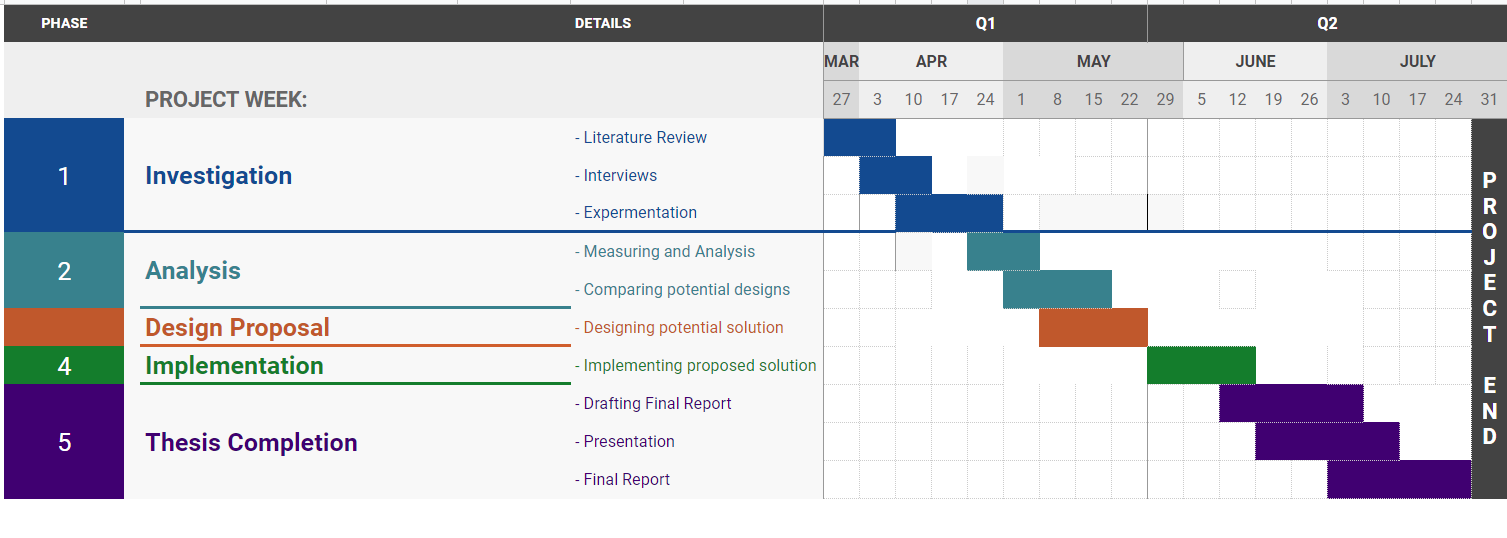
\includegraphics[scale=0.65]{Images/timeline.png}
   \end{center}

\bibliography{sources}
\bibliographystyle{IEEEtran}
\end{document}
